
\chapter{Experiments} % Main chapter title

\label{ch:05} % Change X to a consecutive number; for referencing this chapter elsewhere, use \ref{ChapterX}
The experiments are performed on two normal inference tasks: normal inference based on depth image and guided normal inference based on RGB-D image. Prior works for normal estimation using very deep networks. For a single object surface normal detection as stated in this thesis, the given methods has a similar performance but only with $ 1/10 $ size.

The model is trained with PyTorch 1.10.2, CUDA 10.2.89, GPU with single NVIDIA GEFORCE GTX 1080Ti.


%% nnnn exp
\section{Surface Normal Inference based on Depth Map}
The goal of surface normal inference is to calculate the tangent surface normal map $ N $ from a single depth map $ D $. A network named Gated Convolution Neural Network (GCNN) is trained and is compared with similar approaches.

\subsection{Compared Approaches}


\subsection{Training Details}
The network (see \ref{gcnn}) is trained on stated dataset in Chapter \ref{ch:04}. It has two versions, the L-size $ 512\times512\times3 $ and the  S-size $ 128\times128\times3 $. For the L-size model, it uses batch size 8 for 3500 iterations. For the S-size model, it uses batch size 32 for 6000 iterations. Both sizes use Adam optimizer \cite{adam} with a learning rate of $ 1\times10^{-3} $, penalty-l2 loss(see \ref{sec:loss}). The output is directly the tangent normal in range $ \left[-1,1\right] $. The output and input has the same shape.


\subsection{Qualitative Evaluation}

The evaluation visualization on dataset ``synthetic50-5" (see \ref{ch:04}) dataset is shown in Figure \ref{fig:gcnn-eval-synthetic}. It compares the results with method xxx, for both smooth and highly detailed cases. In all the cases, the angle errors are very close. The test-cases are based on test point cloud in ``synthetic50-5". 

The model is supposed to used on any image size since it has no fully-connected layers (dense layers). Two size of models are based on exactly the same architecture. 

%% a detailed analyis of this figure
It is 




The evaluation visualization on real dataset is shown in Figure \ref{fig:gcnn-eval-real}
\begin{figure}[h!]
	\centering
	\begin{subfigure}[b]{0.24\linewidth}
		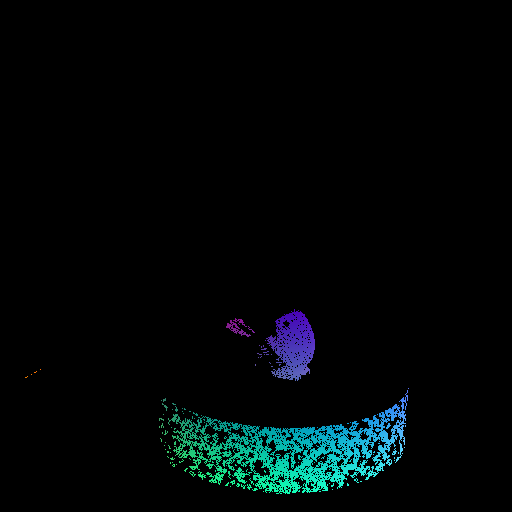
\includegraphics[width=\linewidth]{./Figures/gcnn-real/fancy_eval_1_point_cloud_noise.png}
		\caption{point cloud}
	\end{subfigure}
	\begin{subfigure}[b]{0.24\linewidth}
		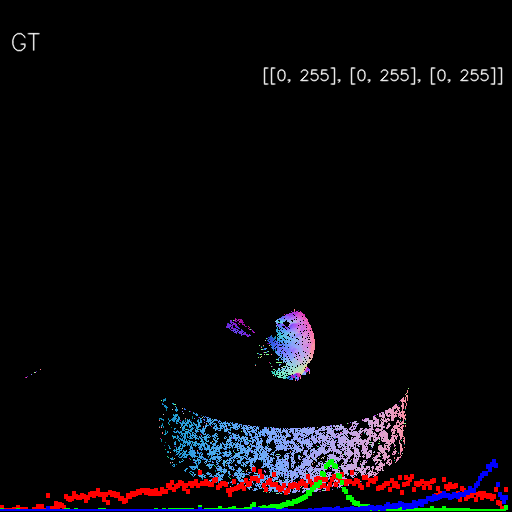
\includegraphics[width=\linewidth]{./Figures/gcnn-real/fancy_eval_1_groundtruth.png}
		\caption{ground-truth}
	\end{subfigure}
	\begin{subfigure}[b]{0.24\linewidth}
		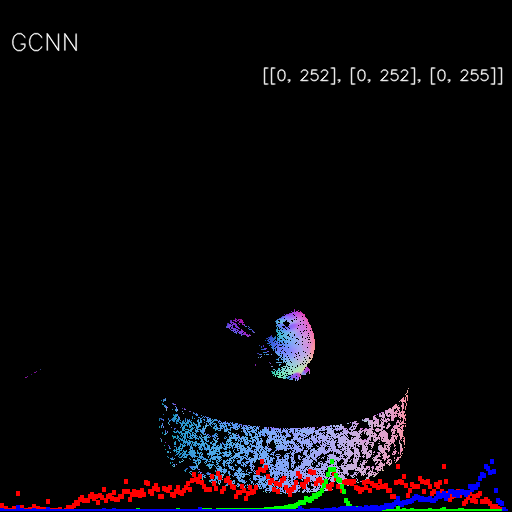
\includegraphics[width=\linewidth]{./Figures/gcnn-real/fancy_eval_1_normal_GCNN.png}
		\caption{GCNN}
	\end{subfigure}
	\begin{subfigure}[b]{0.24\linewidth}
		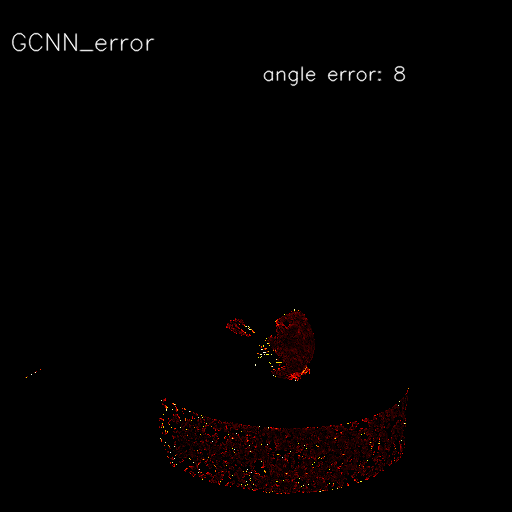
\includegraphics[width=\linewidth]{./Figures/gcnn-real/fancy_eval_1_error_GCNN.png}
		\caption{Angle Error}
	\end{subfigure}
	\caption{Evaluation on Real Dataset}
	\label{fig:gcnn-eval-real}
\end{figure}



\subsection{Quantitative Evaluation }





The evaluation result on test scenes is shown in Figure \ref{fig:scatter-gcnn}.
The GCNN based method has angle error between 5 to 15 degrees in both type of inputs. The error trends to higher with point number decrease. It is because the less points in the point cloud, the more detail is hided due to the insufficient of resolution. Therefore the recorded surface based on the point cloud is more coarse, which also increase the difficulty of the normal inference.

\begin{figure}[h!]
	\centering
	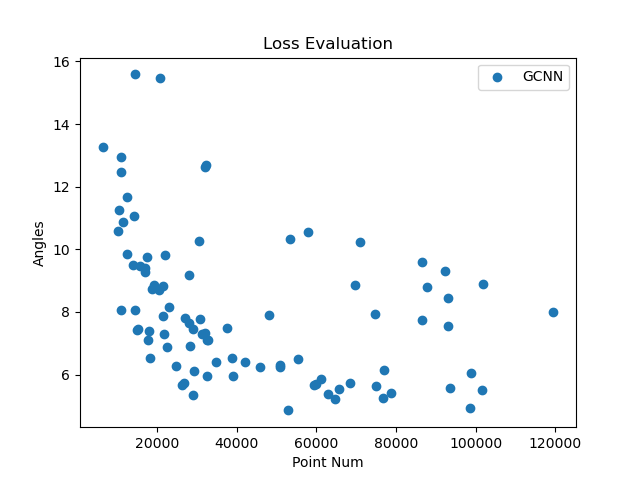
\includegraphics[width=.4\textwidth]{./Figures/scatter-gcnn-no-noise.png}
	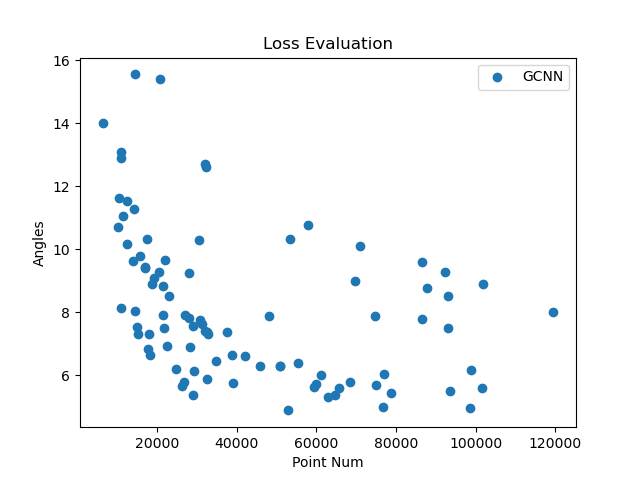
\includegraphics[width=.4\textwidth]{./Figures/scatter-gcnn-noised.png}
	\caption{Evaluation of average angular loss on the whole test dataset with 90 scenes. The x-axis indicates the point number, the y-axis indicates the angles. The \textbf{Left} one using point cloud without noise, the \textbf{right} one has noise.}
	\label{fig:scatter-gcnn}
\end{figure}




\subsection{Speed}


%% resng
\section{Guided Gated Convolution Neural Network for Normal Inference }

The inference result of guided-GCNN model is shown in Figure \ref{fig:ng-eval-synthetic}. With adding the information of a gray-scale image, the model is able to sharpen the details over the whole scene. 

\begin{figure}[h!]
	\centering
	\begin{subfigure}[b]{0.19\linewidth}
		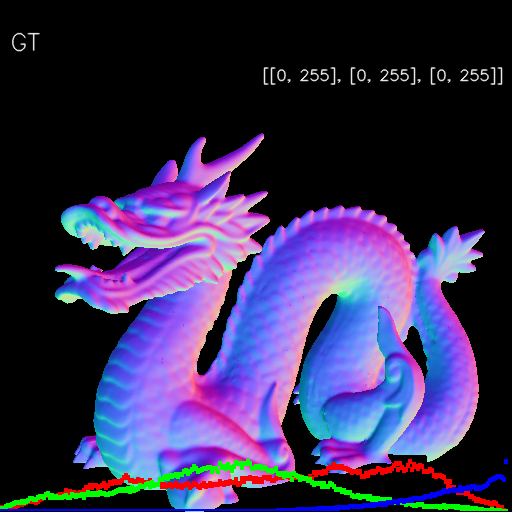
\includegraphics[width=\linewidth]{./Figures/ng-synthetic/fancy_eval_3_groundtruth.png}
		\caption{GT}
	\end{subfigure}
	\begin{subfigure}[b]{0.19\linewidth}
		\includegraphics[width=\linewidth]{./Figures/ng-synthetic/fancy_eval_3_normal_NG.png}
		\caption{g-GCNN}
	\end{subfigure}
	\begin{subfigure}[b]{0.19\linewidth}
		\includegraphics[width=\linewidth]{./Figures/ng-synthetic/fancy_eval_3_error_NG.png}
		\caption{Angle Error}
	\end{subfigure}
	\begin{subfigure}[b]{0.19\linewidth}
		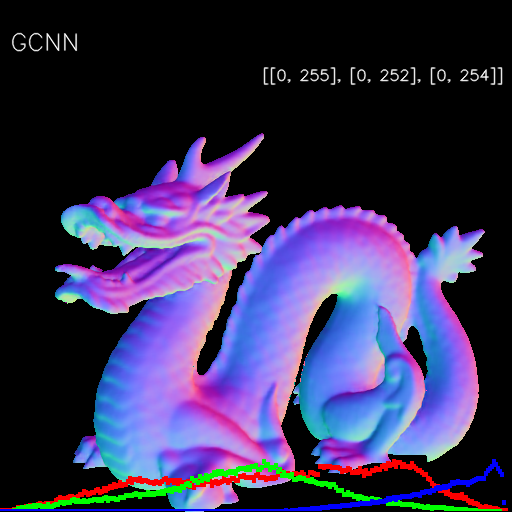
\includegraphics[width=\linewidth]{./Figures/gcnn-synthetic/fancy_eval_3_normal_GCNN.png}
		\caption{GCNN}
	\end{subfigure}
	\begin{subfigure}[b]{0.19\linewidth}
		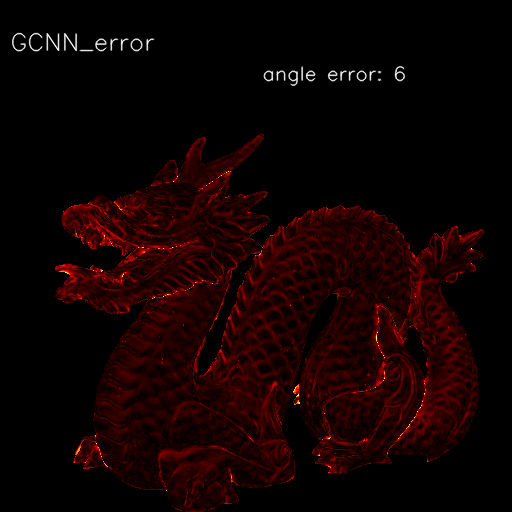
\includegraphics[width=\linewidth]{./Figures/gcnn-synthetic/fancy_eval_3_error_GCNN.png}
		\caption{Angle Error}
	\end{subfigure}
	\caption{guided-GCNN Normal Inference on Synthetic Dataset (object: dragon). GCNN result is shown on (d) and (e) as comparison.}
	\label{fig:ng-eval-synthetic}
\end{figure}



\section{Guided Gated Convolution Neural Network for Normal Inference }

From the Figure \ref{fig:normal-histo-diff} we can observe the normal difference between ground-truth and GCNN predicted normals in another dimension. It separates the interval $ \left[ -1,1 \right] $, which is exactly the range of normal vector, to 256 sections. Then it counts the number of points locates in each section for 3 axes.  The 3 axes are fitted quit well in most of interval but other than $ \left[ -0.25,0.25 \right] $ for x and y axes and  interval close to $ -1 $ for z axis. Therefore a further constraint can be considered to the loss function related to the normal difference shown in this figure.

It is faulty that almost no normal has -1 z-component in GCNN predicted normal map. The reason?
\begin{figure}[h!]
	\centering
	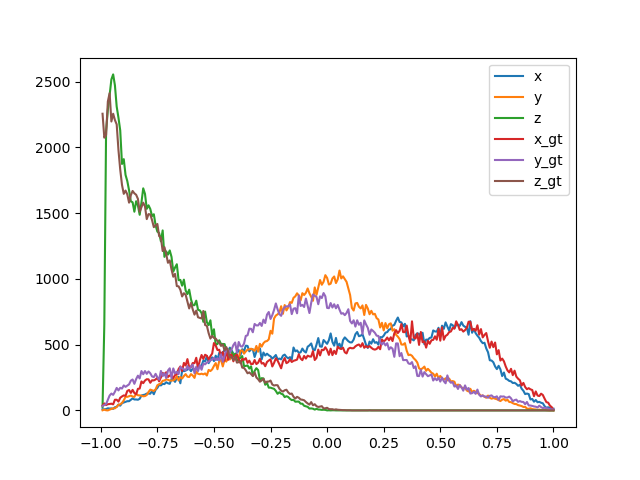
\includegraphics[width=\linewidth]{./Figures/normal-histo-diff.png}
	\caption{The normal difference of between GCNN and ground-truth in x, y, z-axis respectively. The y axis indicates the number of points, x axis indicates the value of normal in x/y/z axis. (The chart is based on the "dragon" scene showing above)}
	\label{fig:normal-histo-diff}
\end{figure}


\newpage 
\section{model comparison}
This section evaluates the proposed models with the neighbor-based model and make comparison with each other.

\begin{figure}[h!]
	\centering
	\begin{subfigure}[b]{0.24\linewidth}
		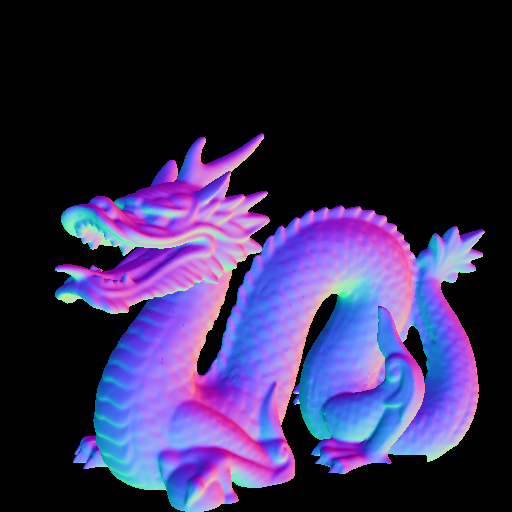
\includegraphics[width=\linewidth]{./Figures/comparison/fancy_eval_3_groundtruth.png}
		\caption{ground-truth}
	\end{subfigure}
	\begin{subfigure}[b]{0.24\linewidth}
		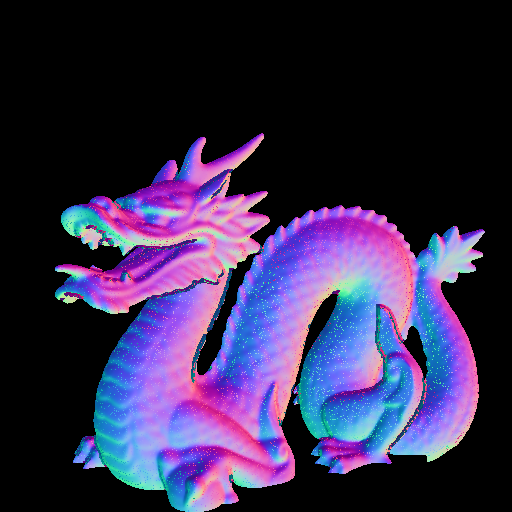
\includegraphics[width=\linewidth]{./Figures/comparison/fancy_eval_3_normal_svd.png}
		\caption{SVD}
	\end{subfigure}
	\begin{subfigure}[b]{0.24\linewidth}
		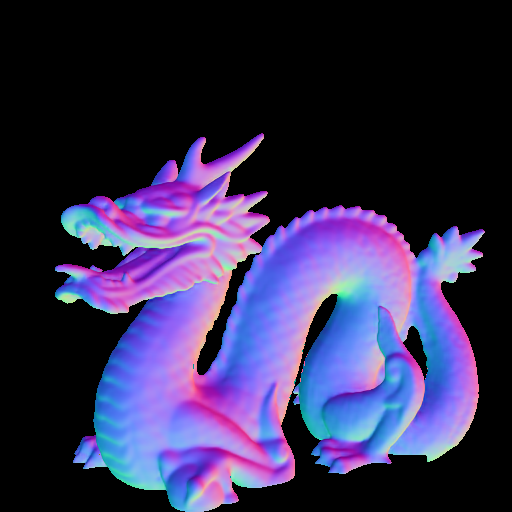
\includegraphics[width=\linewidth]{./Figures/comparison/fancy_eval_3_normal_GCNN.png}
		\caption{GCNN}
	\end{subfigure}
	\begin{subfigure}[b]{0.24\linewidth}
		\includegraphics[width=\linewidth]{./Figures/comparison/fancy_eval_3_normal_NG.png}
		\caption{guided-GCNN}
	\end{subfigure}
	
	\begin{subfigure}[b]{0.3\linewidth}
		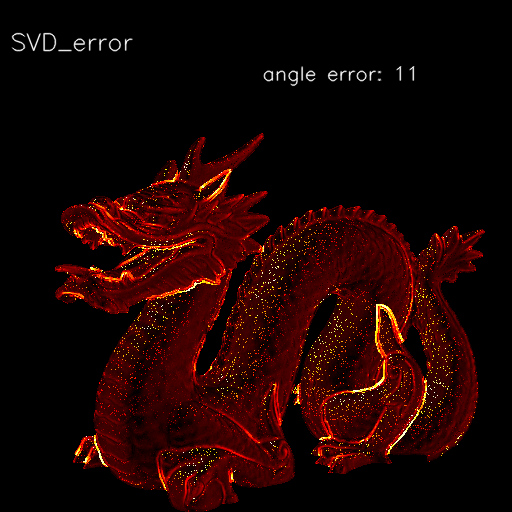
\includegraphics[width=\linewidth]{./Figures/comparison/fancy_eval_3_error_SVD.png}
		\caption{Error}
	\end{subfigure}
	\begin{subfigure}[b]{0.3\linewidth}
		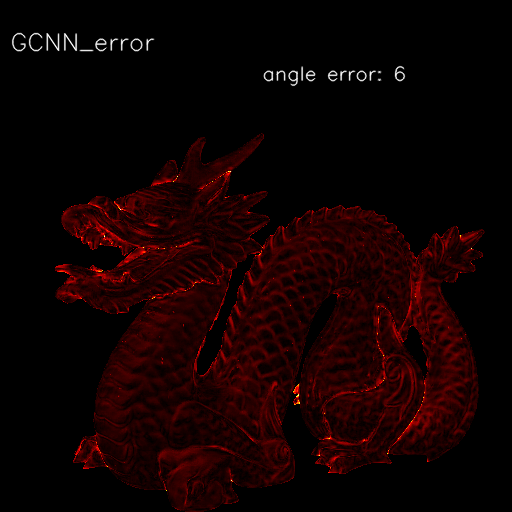
\includegraphics[width=\linewidth]{./Figures/comparison/fancy_eval_3_error_GCNN.png}
		\caption{Error}
	\end{subfigure}
	\begin{subfigure}[b]{0.3\linewidth}
		\includegraphics[width=\linewidth]{./Figures/comparison/fancy_eval_3_error_NG.png}
		\caption{Error}
	\end{subfigure}
	
	\caption{Normal Inference on different models with errors. (object: dragon)}
	\label{fig:eval-svd}
\end{figure}
